\subsection{Comparación entre Compiladores}
Un compilador no es mas que un programa que basicamente toma el codigo C
y lo traduce a codigo de maquina. Existen varios para C, tales como como GCC (el cual se usa en gran parte de este trabajo), Clang y el Compilador de Intel.
Lo que hicimos en este experimento fue compilar los filtros con GCC y Clang en sus versiones 5.3.1 y 3.8.0 respectivamente, para luego realizar la comparación.
%Lo que vamos a hacer es compilar el codigo con Clang/GCC y ver si encontramos diferencias.Para comparar, se van a usar la version 4.8.4 de GCC y la 3.4 de Clang.
%Para realizar la comparacion, vamos a compilar el TP con GCC y luego con Clang.
%Para empezar, vamos a comparar con optimizacion nula
Nuestra hipótesis para este experimento es que el compilador de GCC optimice más el código producido que Clang, ya que en caso contrario, este último estaría instalado por defecto
en muchos de los sistemas operativos existentes en lugar de GCC (teniendo en cuenta las muchas otras razones por las que puede no ser el caso).


Aqui el grafico de GCC sin optimización

\begin{figure}[H]
    \centering
    \begin{floatrow}
      \ffigbox[\FBwidth]{\caption{Filtros con GCC -O0}}{%
        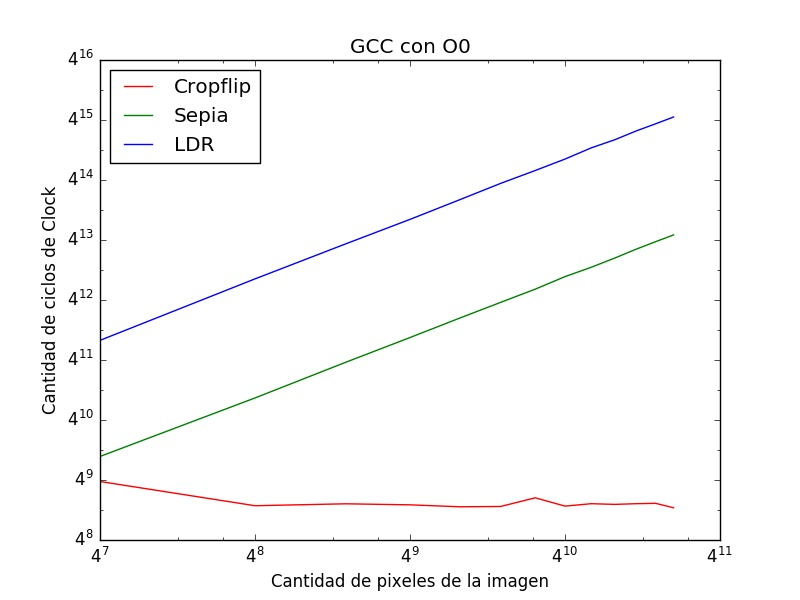
\includegraphics[scale=.55]{./imagenes/GCC0.jpg}
      }
    \end{floatrow}
\end{figure}


Aca vemos que Cropflip, que es el filtro más rápido, empieza tomando $4^9$ ciclos de reloj en la imagen más chica y finaliza cerca de la mitad entre $4^8$ y $4^9$.
Los otros dos filtros alcanzan hasta $4^13$ y $4^15$ ciclos de reloj.

Aqui el grafico de Clang

\begin{figure}[H]
    \centering
    \begin{floatrow}
      \ffigbox[\FBwidth]{\caption{Filtros con Clang -O0}}{%
        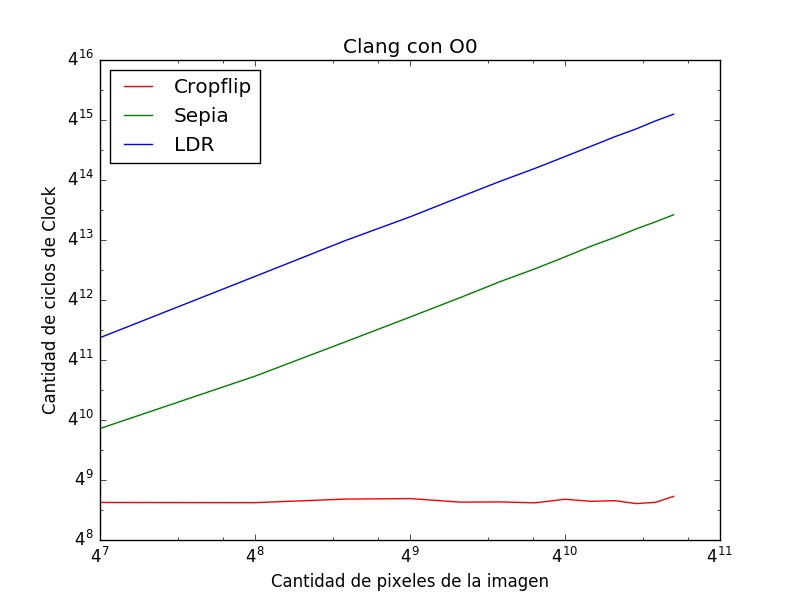
\includegraphics[scale=.55]{./imagenes/Clang0.jpg}
      }
    \end{floatrow}
\end{figure}

Tras este gráfico, observamos que las diferencias de LDR y Sepia son casi nulas entre los compiladores, sin embargo Cropflip tiene la diferencia de que es más
lineal en cuanto a ciclos de reloj sobre tamaño de la imagen.


Ahora, vamos a repetir el mismo experimento pero variando las flags, esta vez vamos a usar 03. Como hipotesis, esperamos ver un comportamiento similar al visto en O0.
\begin{figure}[H]
    \centering
    \begin{floatrow}
      \ffigbox[\FBwidth]{\caption{Filtros con GCC -O3}}{%
        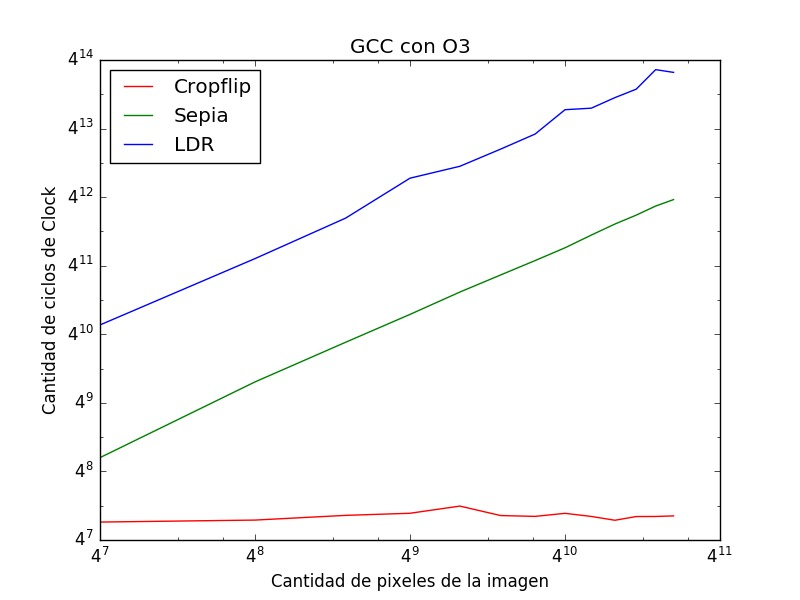
\includegraphics[scale=.55]{./imagenes/GCC3.jpg}
      }
    \end{floatrow}
\end{figure}


\begin{figure}[H]
    \centering
    \begin{floatrow}
      \ffigbox[\FBwidth]{\caption{Filtros con Clang -O3}}{%
        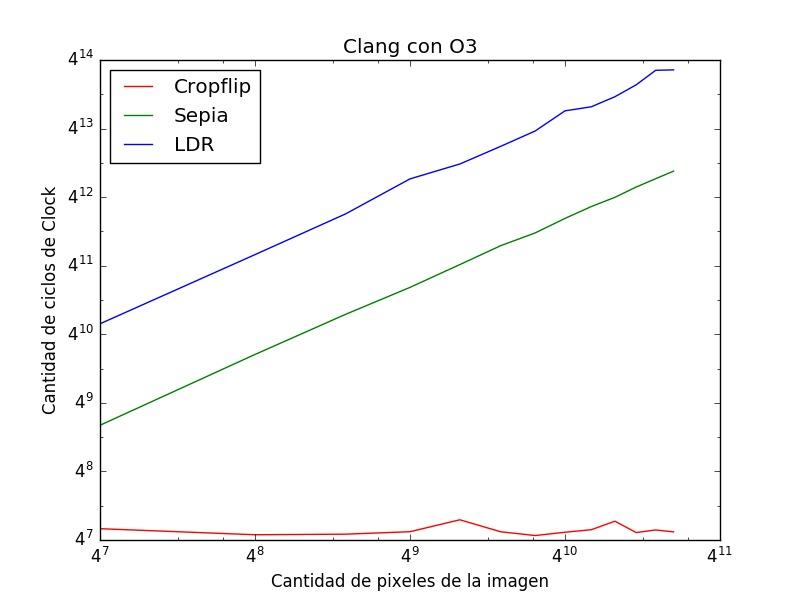
\includegraphics[scale=.55]{./imagenes/Clang3.jpg}
      }
    \end{floatrow}
\end{figure}

Ciertamente, se observó lo esperado. Tienen un comportamiento muy similar más allá de los flags de optimización. Podemos entender entonces que la desición
sobre usar un compilador u otro quedaría simplemente por preferencia y no por performance.
